\documentclass[a4paper,10pt]{article}
\usepackage[top=2cm, bottom=2cm, left=2cm , right=2cm]{geometry}
\usepackage[utf8]{inputenc}
\usepackage{fancyhdr}
\pagestyle{fancy}
\usepackage{graphicx}
\usepackage{amsfonts}
\usepackage{fourier}
\usepackage{wasysym}

\title{}
\author{Hicham Benjelloun}
\date{}

\pdfinfo{%
  /Title    ()
  /Author   ()
  /Creator  ()
  /Producer ()
  /Subject  ()
  /Keywords ()
}

\begin{document}
\lhead{Hicham Benjelloun - 1A INFO}
\rhead{Rendu le 14/06/2013}
\begin{figure}[!h]
 \centering
 
\includegraphics[scale=0.6]{logo.jpg}
\end{figure}

\begin{center}
 {\Large \textbf{Rapport de projet}} \\
 \textit{Grand Prix} \\
\end{center}
\textbf{Encadrants de projet :} Hidane Moncef et Christophe Rosenberger.

\renewcommand{\contentsname}{Table des matières}
\tableofcontents

\section{Introdution}

Ce projet consiste en la réalisation d'un pilote en langage C pour GNU/Linux. Un pilote est un programme qui, en communication avec un gestionnaire de course \textit{via} les entrée/sortie standards, va envoyer successivement des accélérations
pour rejoindre un point d'arrivée, en respectant un certain nombre de contraintes qui sont détaillées dans l'énoncé du sujet écrit par Julien Gosme.
\\
\\
En particulier, les objectifs de ce travail sont de réaliser un pilote robuste qui respecte les conditions imposées par le gestionnaire de course et qui relie un point de départ à un point d'arrivée en un nombre de tours de jeu que l'on peut espérer
optimal, et ce, pour tout type de carte\footnote{Éventuellement non connexe}.

\section{Définitions et notations}
Avant de comprendre ce qu'est un bon pilote\footnote{Un pilote qui gagne souvent les courses !}, il est naturel de se demander quelle est sa définition\footnote{Et donc comment le représenter} et
comment ce dernier peut se comporter face à une carte quelconque. Le but de cette partie est donc de formaliser le problème en vue de poser des bases solides pour l'implémentation du programme.

\subsection{Carte}
Un carte de de taille $h\times w$ est une matrice de caractères parmi \{ \verb # ,\verb ~ ,\verb . ,\verb = \}.
\subsection{Pilote}
Un pilote est la donnée d'un vecteur position $p$, d'une vitesse $v$ et du nombre de boosts $b$ dont il dispose. Le triplet $(p,v,b)$ consitue \textbf{un état unique du pilote}.
\subsection{Voisinage}
Une fonction de voisinage $\Phi$ est une fonction donnant, pour tout état $e=(p,v,b)$ de pilote, un ensemble $\Phi(e)$ d'états accessibles à partir de $e$.
On construit ce voisinage à partir des contraintes imposées par le gestionnaire : on parcourt la liste des accélérations possibles à partir de $e$ et on regarde celles qui mènent vers un état correct.

\section{Structures de données}

Les principales structures de données utilisées dans ce projet sont les suivantes :\\
\subsection{Map} Représentation d'une carte par un tableau 2D de caractères. \\
\begin{figure}[!h]
 \begin{verbatim}
................................
................................
................................
................................
..#########################==...
..#########################==...
..#########################==...
..#########################==...
..#########################==...
..#########################==...
..#########################==...
................................
................................
................................
................................
................................
\end{verbatim}
\end{figure}
\\
\textbf{Exemple} La carte \textit{Droit au but} fournie avec le gestionnaire de course \\
\subsection{Vertex} Représentation d'un sommet d'un graphe. Contient un élément, une clef et un pointeur vers un prédecesseur.
\subsection{Graph} Représentation d'un graphe. J'ai choisi d'implémenter cette structure par un tableau 4D de pointeurs sur des sommets pour permettre un accès en temps constant à un état d'un pilote à partir d'un autre.
Cette représentation facilite grandement la construction du voisinage $\Phi(e)$ d'un état $e$.
\begin{figure}[!h]
\centering
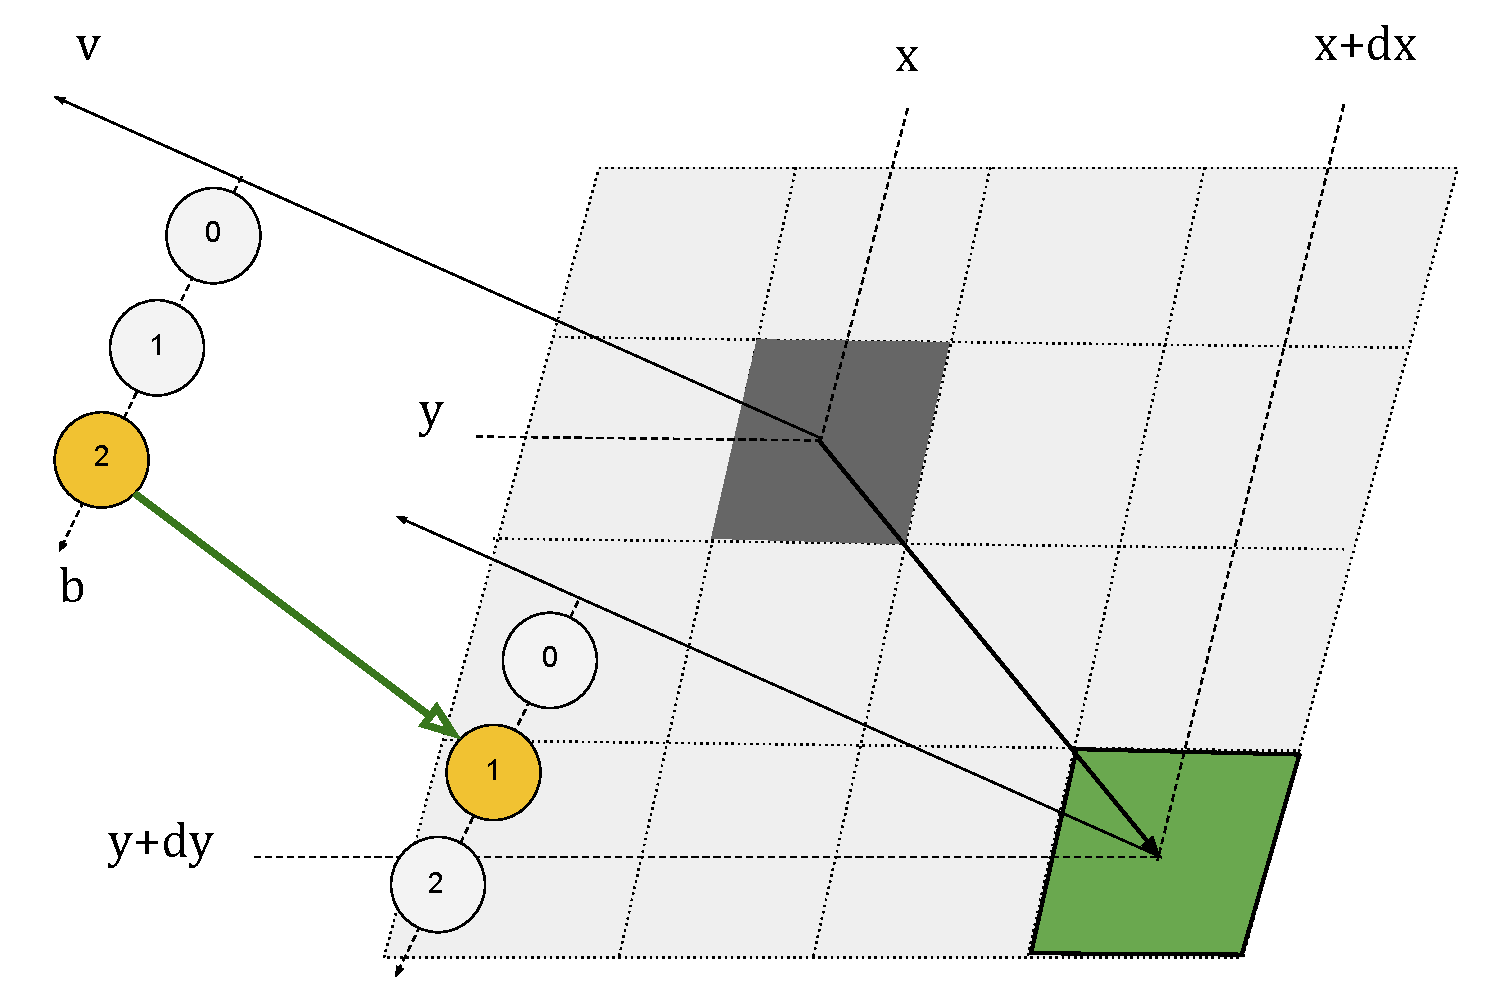
\includegraphics[scale=0.5]{graph.pdf}
\caption{Représentation du graphe des états possibles}
\end{figure}
\noindent
Dans cette représentation, un état $e$ est accessible dans le graphe $G$ en temps constant par ses paramètres : $e=G[x][y][v][b]$\footnote{Attention, une vitesse $v$ est représentée ici par son index, donc un seul entier ; ceci étant
possible du fait que l'ensemble des vitesses de norme $\leq$ à $5$ est fini et donc qu'on peut le numéroter}.
Un accéleration $a$ permettant d'atteindre une vitesse $v'$ à partir de $v$ l'état suivant de $e$ par a est donné par $G[x+dx][y+dy][v'][b']$ où $dx$ et $dy$ sont les composantes de la vitesse $v'$ et où
$b'=b-1$ si la norme de $a$ est supérieure à $2$, $b'=b$ sinon.
\\
\subsection{Path} Chemin à partir d'un sommet renvoyé par l'algorithme de Dijkstra détaillé plus loin. Le chemin correspond à une liste de sommets. 
\\
Se référer aux fichiers d'en-tête pour plus de précisions concernant l'implémentation de ces structures.

\section{Algorithme implémenté}
\subsection{Calcul d'un plus court chemin}
Parmi les différentes stratégies qui peuvent être mises en place pour trouver un chemin de longueur optimale, j'ai choisi d'implémenter une version
\footnote{Originellement, cet algorithme très simple ne faisait que calculer la longueur du plus court chemin dans un graphe. Une légère modification nous permet de récupérer ce chemin}
de l'algorithme de Dijkstra pour trouver le plus court chemin dans le graphe des états possibles du pilote.
\\
\\
Cet algorithme, détaillé ci-dessous, permet de calculer le plus court chemin dans le graphe des états possibles d'un pilote en temps polynômial.
L'extraction du minimum, qui se fait en $O(log_{2}(n))$ repose sur l'utilisation des tas de Fibonacci, structure de donnée conçue par Michael L. Fredman et Robert E. Tarjan en 1984 pour optimiser l'algorithme de Dijkstra.
Pour cette partie\footnote{Relativement complexe} seulement, j'ai utilisé une implémentation disponible à l'adresse suivante :
\begin{verbatim}
 http://resnet.uoregon.edu/~gurney_j/jmpc/fib.html
\end{verbatim}

\paragraph{Description de l'algorithme de Dijsktra}

Soit un graphe $G$ de fonction de voisinage $\Phi$ et soit un point de départ $a$.

\begin{itemize}
 \item [E1.] Pour tout sommet $s$ du graphe des états $G$, faire $d(s)\leftarrow\infty$
 \item [E2.] $d(a)\leftarrow 0$
 \item[E3.] Ajouter $a$ au tas $F$.
 \item[E4.] Tant que $F\neq\emptyset$, extraire le sommet $u$ de distance minimale et mettre à jour chaque $v\in\Phi(u)$ :
 \begin{itemize}
  \item [E4.1] Si $d(v)>d(u)+1$, faire $d(v)\leftarrow d(u)+1$ et $pred(v)\leftarrow u$.
  \item[E4.2] Si $v$ est un état correspondant à une position d'arrivée, on peut retourner directement ce sommet.
 \end{itemize}
\end{itemize}

\paragraph{Construction du chemin}
Le chemin se construit facilement en remontant à partir du sommet renvoyé par l'algorithme précédent, vu qu'on a stocké dans chaque sommet son prédecesseur.

\subsection{Mise à jour dynamique du chemin}
Il faut garder à l'esprit que la course se déroule en présence d'autre pilotes et que l'on ne peut bien évidemment pas, à un instant donné, aller vers une case occupée par un autre pilote.
Cela implique qu'il faut vérifier à chaque tour de jeu la validité de l'accélération que l'on s'apprête à envoyer au gestionnaire.

\begin{itemize}
 \item [E1.] Si on n'a pas de chemin, on construit un plus court chemin jusqu'à l'arrivée.
 \item[E2.] Tant que la partie n'est pas terminée, on récupère l'état suivant du pilote à partir du chemin précédemment calculé et on teste sa validité
 \begin{itemize}
  \item [E2.1] Si le coup est valide, on envoie l'accélération au gestionnaire de course.
  \item[E2.2] Si le coup est non valide, on reconstruit un nouveau chemin optimal en retirant les états de $\Phi(e)$ dont la position coïncide avec au moins l'une des positions des autres pilotes. 
    On obtient un nouvel ensemble $\Phi'(e)$.
      \item[E2.2.1] Si $\Phi'(e)$ est vide, alors le pilote ne peut donner une autre accélération lui permettant de continuer et le gestionnaire l'arrête. On recommence depuis (E1) à vitesse nulle.
      \item[E2.2.2] Si $\Phi'(e)$ contient au moins un élément, on recalcule donc un nouveau chemin optimal à partir de la position courante et on continue à partir de (E2.1).
 \end{itemize}
 
Cette mise à jour simple est détaillé dans le diagramme ci-dessous :

\begin{figure}[!h]
\centering
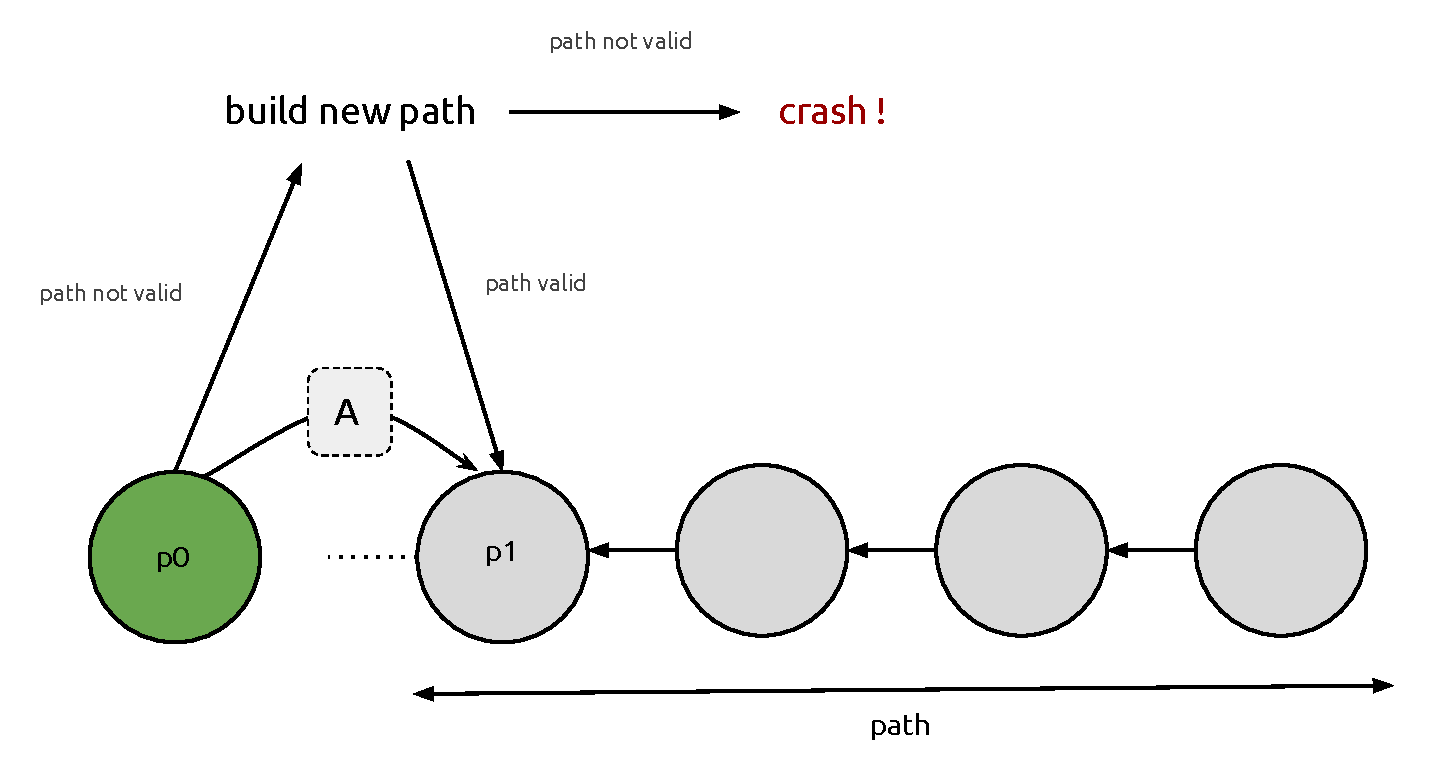
\includegraphics[scale=0.6]{game.pdf}
\caption{Mise à jour dynamique du chemin}
\end{figure}

\section{Conclusion}

Ce projet a été l'occasion d'implémenter et d'adapter l'algorithme de Dijsktra qui donne à partir d'un graphe des états possibles d'un pilote, un chemin optimal reliant ce même pilote à l'arrivée, sur tout type de carte
\footnote{Il faut bien évidemment qu'au moins un chemin reliant le départ et l'arrivée existe}.

Le pilote ainsi obtenu permet de calculer très rapidement un chemin optimal jusqu'à l'arrivée, pour des cartes de taille raisonnable. Il s'adapte en fonction de ses adversaires, en réévaluant le chemin si nécessaire.
À titre d'information, voici quelques résultats obtenus\footnote{En nombre de tours de jeu} sur les cartes officielles, en comparaison avec les pilotes GPDriverOne et GPDriverTwo fournis avec le gestionnaire de course.
\\
\\
\begin{center}

\begin{tabular}{|c|c|c|c|}
  \hline
  Carte/Pilote& GPDriverOne & GPDriverTwo & Mon pilote \\
  \hline
  Droit au but &13 & 9 & 6 \\
  Virages &112 & 75 & 39 \\
  Virages et sable & 430 & 354& 41\\
  Serpent & 257 & 77& 33\\
  \hline
\end{tabular}
\end{center}


\end{itemize}










\end{document}
